\documentclass[aspectratio=169%可调屏宽比16:9(169),4:3(43)
,serif,mathserif]{beamer}
\mode<presentation>{
%\usetheme{default}
%\usetheme{AnnArbor}
%\usetheme{Antibes}
%\usetheme{Bergen}
%\usetheme{Berkeley}
%\usetheme{Berlin}
%\usetheme{Boadilla}
%\usetheme{CambridgeUS}
%\usetheme{Copenhagen}
%\usetheme{Darmstadt}
%\usetheme{Dresden}
%\usetheme{Frankfurt}
%\usetheme{Goettingen}
%\usetheme{Hannover}
%\usetheme{Ilmenau}
%\usetheme{JuanLesPins}
%\usetheme{Luebeck}
\usetheme{Madrid}
%\usetheme{Malmoe}
%\usetheme{Marburg}
%\usetheme{Montpellier}
%\usetheme{PaloAlto}
%\usetheme{Pittsburgh}
%\usetheme{Rochester}
%\usetheme{Singapore}
%\usetheme{Szeged}
%\usetheme{Warsaw}
% As well as themes, the Beamer class has a number of color themes
% for any slide theme. Uncomment each of these in turn to see how it
% changes the colors of your current slide theme.
%\usecolortheme{albatross}
%\usecolortheme{beaver}
%\usecolortheme{beetle}
%\usecolortheme{crane}
%\usecolortheme{dolphin}
%\usecolortheme{dove}
%\usecolortheme{fly}
%\usecolortheme{lily}
%\usecolortheme{orchid}
%\usecolortheme{rose}
%\usecolortheme{seagull}
%\usecolortheme{seahorse}
%\usecolortheme{whale}
%\usecolortheme{wolverine}
%\setbeamertemplate{footline} % To remove the footer line in all slides uncomment this line
%\setbeamertemplate{footline}[page number] % To replace the footer line in all slides with a simple slide count uncomment this line
%\setbeamertemplate{navigation symbols}{} % To remove the navigation symbols from the bottom of all slides uncomment this line
}
\usepackage{adjustbox}
\usepackage{hyperref}
\usepackage{indentfirst} 
\usepackage{amsmath, amsfonts, epsfig, xspace}
\usepackage{algorithm,algorithmic}
\usepackage{beamerthemesplit}
\usepackage{booktabs}
\usepackage{bm}
\usepackage{braket}
\usepackage{calligra}
\usepackage[T1]{fontenc}
\usepackage{fontspec}
\usepackage{ctex}
\usepackage{latexsym}
\usepackage{multicol}
\usepackage{multimedia}
\usepackage{calligra} \DeclareMathAlphabet{\mathcalligra}{T1}{calligra}{m}{n} \DeclareFontShape{T1}{calligra}{m}{n}{<->s*[2.2]callig15}{}
\usepackage{pstricks,pst-node}
\usepackage{ragged2e}
\usepackage{setspace}
\usepackage[normal,tight,center]{subfigure}
\setlength{\subfigcapskip}{-.5em}
\setlength{\parindent}{2em}
\begin{document}
\title{Goose: A Meta-Solver for Deep Neural Network Verification} % The short title appears at the bottom of every slide, the full title is only on the title page
\author[Chi~Zhiming]{Reporter:~Chi~Zhiming} % Your name
\institute[ISCAS] % Your institution as it will appear on the bottom of every slide, may be shorthand to save space
{	
	%Lanzhou University \\ % Your institution for the title page
	%\medskip
	%\textit{chizhm16@lzu.edu.cn} % Your email address
}
	\CTEXoptions[today=old]
	\date{\today} % Date, can be changed to a custom date
\begin{frame}[plain]\vspace{1.5em}
\titlepage\vspace{-0.5cm}
%\centerline{\includegraphics[height=0.30\textheight]{logo.png}}
%\hfill 指导教师:xxx
\end{frame}
\begin{frame}{目录}
\tableofcontents
\end{frame}
\AtBeginSection[]
{
\begin{frame}{\tiny}
\frametitle{目录}
\tableofcontents[currentsection]
\end{frame}
}
%----------------------------------------------------------------------------------------
%	PRESENTATION SLIDES
%----------------------------------------------------------------------------------------

%------------------------------------------------
\section{Introduction} % Sections can be created in order to organize your presentation into discrete blocks, all sections and subsections are automatically printed in the table of contents as an overview of the talk
%------------------------------------------------
\begin{frame}
	\frametitle{Contribution}
	\begin{itemize}
		\item Goose, a meta-solver, leverages three key meta-solving techniques, namely, adaptive algorithm selection, probabilistic satisfiability inference, and time interval deepening to implement an adaptive sequential portfolio of solvers for NN verification.
		\item Goose improve 37.7\% across benchmarks and solvers from VNN-COMP'21 and 41.4\% over competition solvers on a 90 select ACAS Xu instances .
	\end{itemize}

\end{frame}

\begin{frame}
	\frametitle{Background}
	VNN-COMP
	\begin{columns}
		\begin{column}{.45\textwidth}
			\begin{itemize}
				\item International Verification of Neural Networks Competition
				\item \href{https://sites.google.com/view/vnn2022}{website link}	
			\end{itemize}
		\end{column}

		\begin{column}{.55\textwidth}
			\begin{figure}[htbp]
				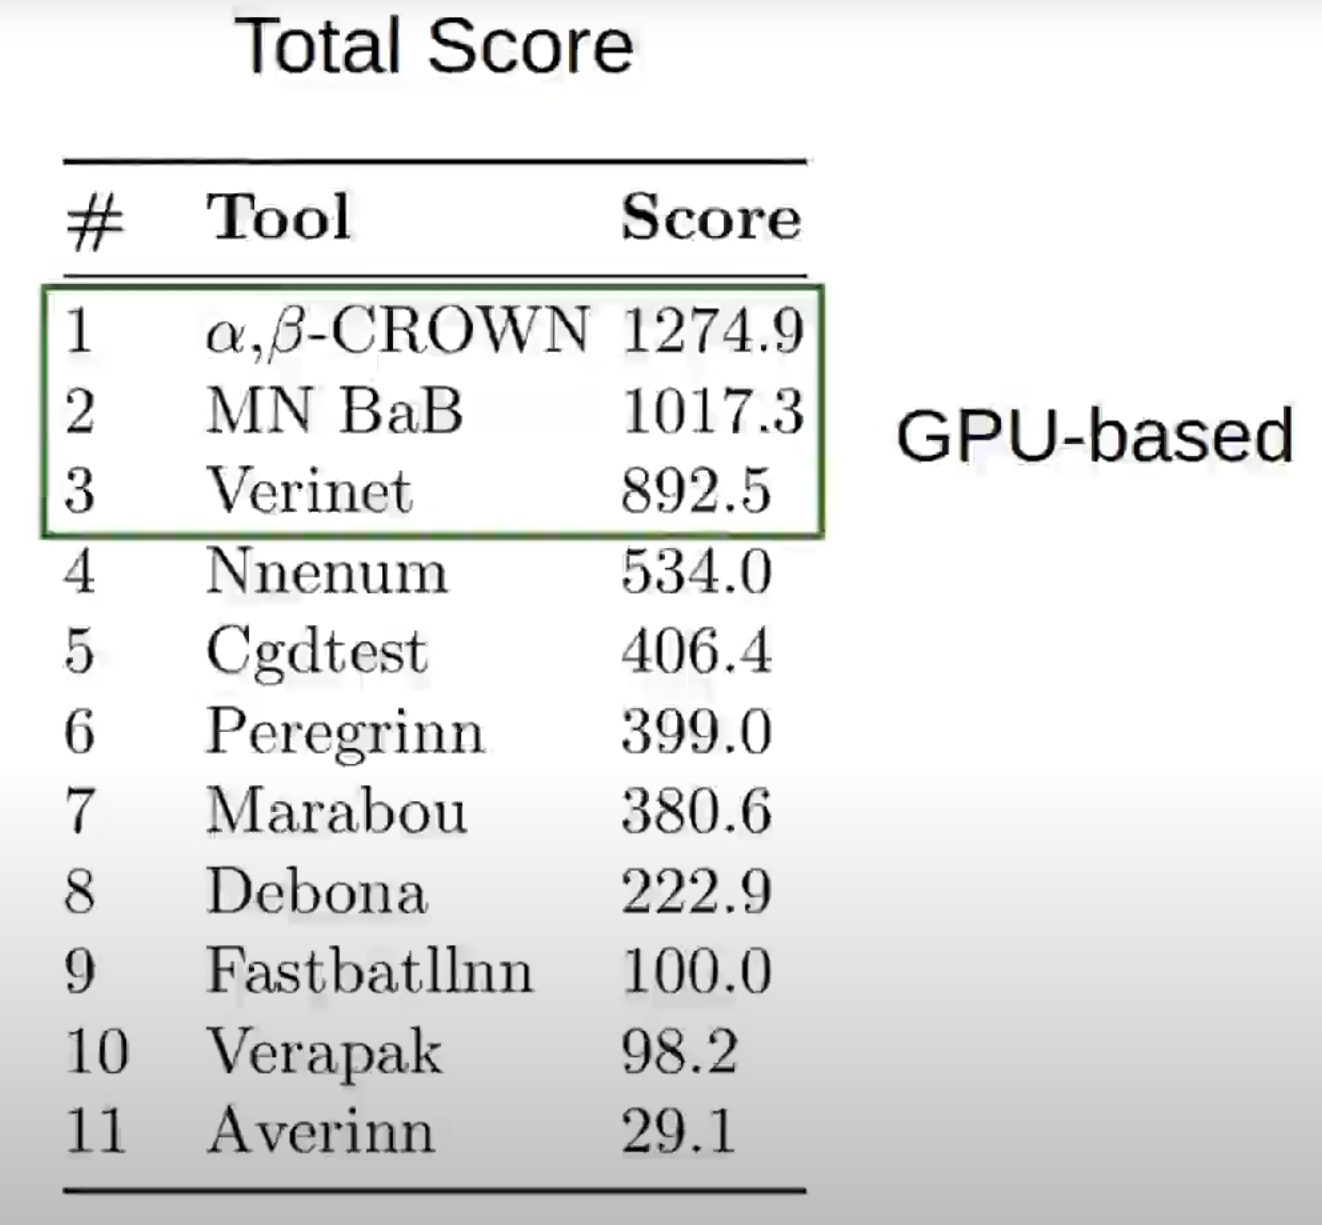
\includegraphics[width=.65\linewidth]{1.png}
			\end{figure}
		\end{column}
	\end{columns}
\end{frame}


% \begin{frame}
% 	\frametitle{Background}
% 	Hybrid SAT solver: Combining both approaches seems promising.
% 	\begin{itemize}
% 		\item use a SLS solver to support a DPLL solver.
% 		\item use information gathered by DPLL solvers on a certain formula to support the search of a SLS solver.
% 		\item SLS and DPLL solvers are supposed to benefit equally from each other.
% 	\end{itemize}	

% \end{frame}

% \begin{frame}
% 	\frametitle{Background}
% 	\begin{itemize}
% 		\item \emph{gNovelty+}:In its core, gNovelty+ utilizes a gradient-based variable score update scheme to calculate candidate variables for the next flip;winner of the random category of the SAT 2007 Competition
% 		\item \emph{March\_ks}:a double look-ahead DPLL solver;the winner of random \textbf{UNSAT} category of the SAT 2007 Competition
% 	\end{itemize}
% \end{frame}


\section{Goose}
\begin{frame}
	\frametitle{Framework}
	\begin{figure}[htbp]
		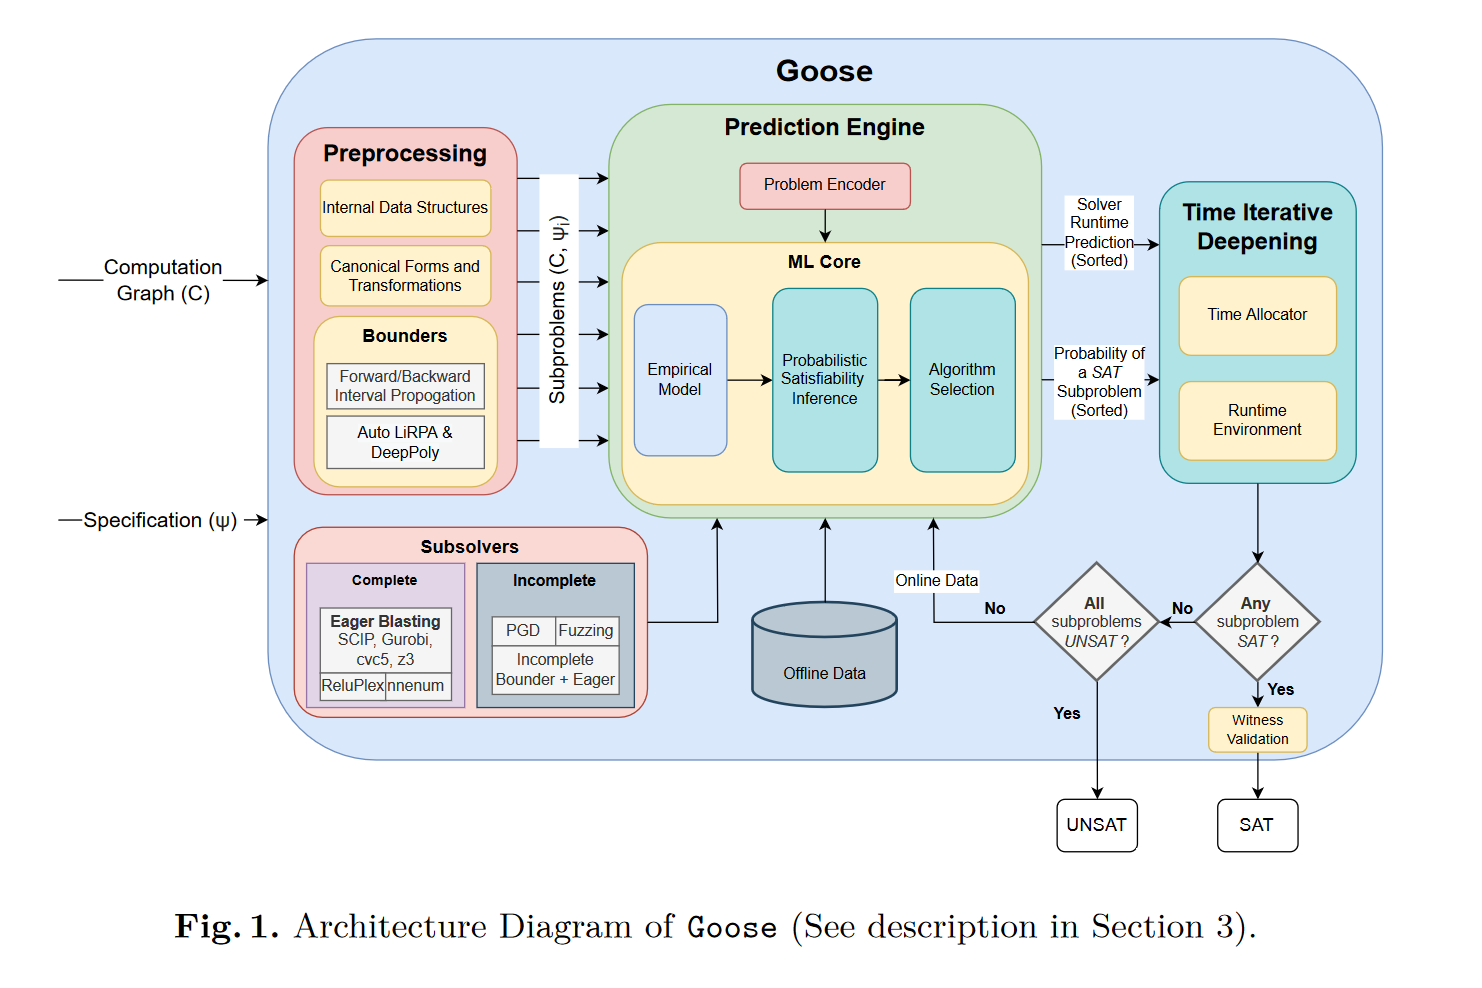
\includegraphics[width=.7\linewidth]{2.png}
	\end{figure}
\end{frame}

\begin{frame}
	\frametitle{Preliminary Study}
	Problem Encoder:
	\begin{itemize}
		\item Goose implements a problem encoder $\xi\left(C ; \psi_i\right)$ to compute \textbf{feature vectors} - a real-valued vector representation of $C, \psi_i$, with 221 dimensions (features).
		\item Network, specification, online information and subproblem features.
	\end{itemize}
	
	Probabilistic Satisfiability Inference
	\begin{itemize}
		\item determine which subproblems to be targeted using decision NN model.
	\end{itemize}

	Algorithm selection:
	\begin{itemize}
		\item determine which solvers should be used decision NN model.
	\end{itemize}
\end{frame}

\begin{frame}
	\frametitle{Pseudocode for Goose}
	\begin{columns}
		\begin{column}{.5\textwidth}
			\begin{figure}[htbp]
				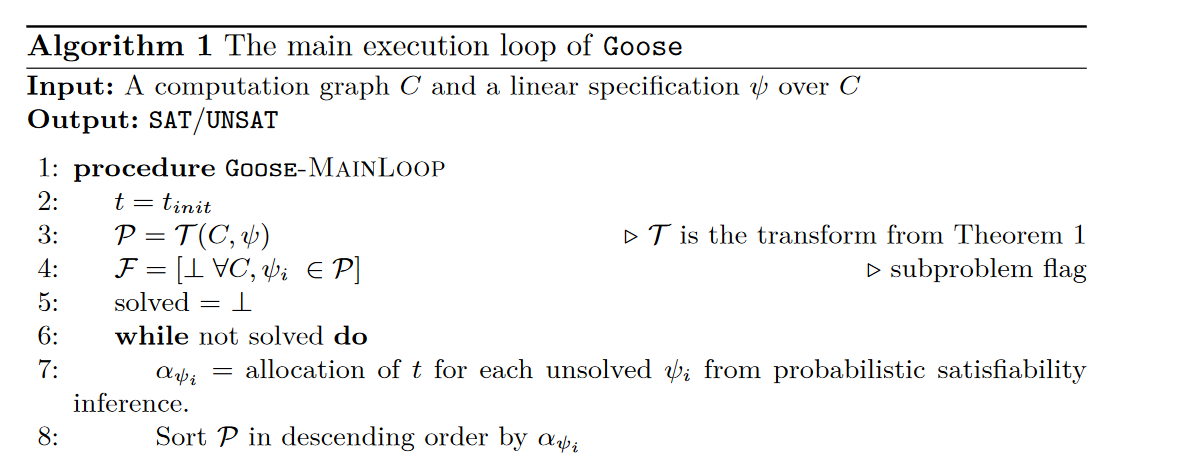
\includegraphics[width=1\linewidth]{3.png}
			\end{figure}
		\end{column}

		\begin{column}{.5\textwidth}
			\begin{figure}[htbp]
				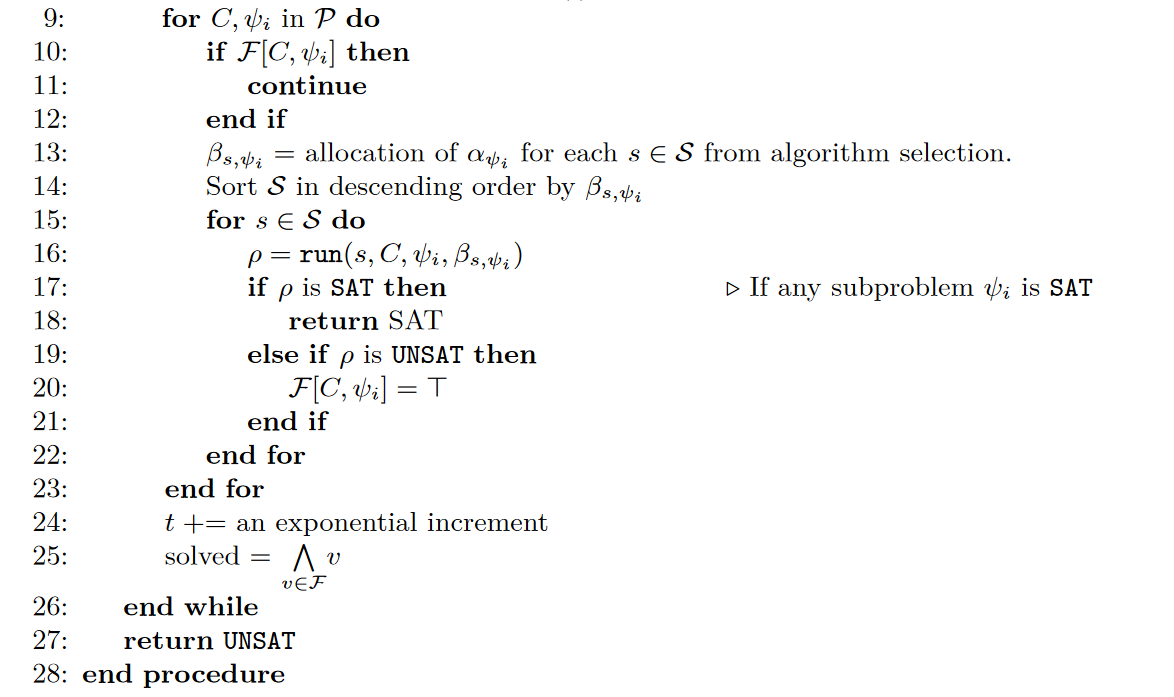
\includegraphics[width=1\linewidth]{4.png}
			\end{figure}
		\end{column}
	\end{columns}
\end{frame}

\section{Experiment}
\begin{frame}
	\frametitle{benchmark of VNN-COMP'21}
	The PAR-2 score of a solver on a benchmark is the wallclock runtime if successful, otherwise twice the wallclock runtime (lower is better).
	\begin{figure}[htbp]
		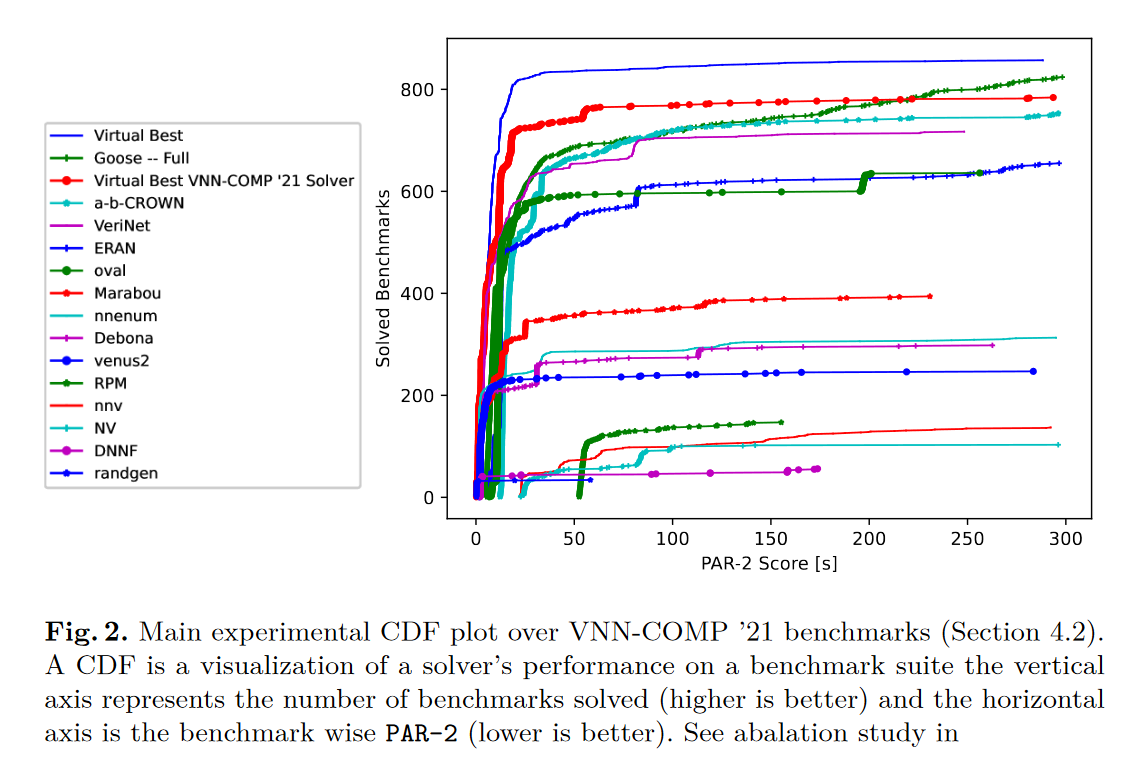
\includegraphics[width=.5\linewidth]{5.png}
	\end{figure}
\end{frame}

\begin{frame}
	\frametitle{benchmark of Acasxu}
	% 做这个实验的原因:When run through the transformer T , 
	% all local robustness queries result in only a single subproblem. 
	% These easier cases do not require the use of our probabilistic satisfiability inference method.

	% 实验数据:We expand this out, to consider all 45 networks, on properties 8 and 10, resulting in 90 new instances with multiple subproblems.
	\begin{figure}[htbp]
		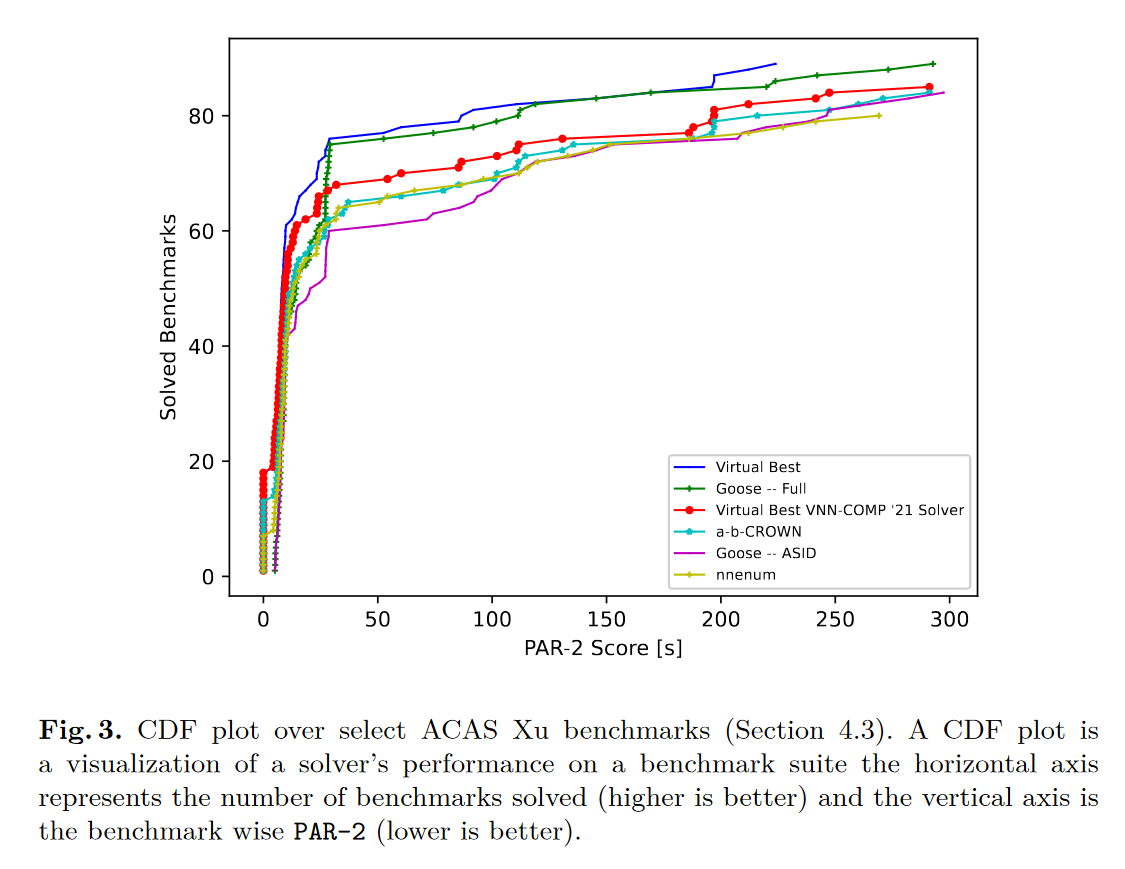
\includegraphics[width=.53\linewidth]{6.png}
	\end{figure}
\end{frame}



% \section{Conclusions and Future Work}

% \begin{frame}
% 	\frametitle{Conclusions}
% 	\begin{itemize}
% 		\item We defined this new term SSP, explained how such SSPs are constructed and how they are used.
% 		\item We implemented our novel approach in the hybrid SAT solver \emph{hybridGM}, utilizing \emph{gNovelty+} as the SLS component and \emph{March\_ks} as the DPLL component.
% 	\end{itemize}
% \end{frame}

% \begin{frame}
% 	\frametitle{Future Work}
% 	\begin{itemize}
% 		\item On uniform random 5- and 7-SAT instances, March ks almost never finds a solution.
% 		\item Dynamically adapt the barrier while hybridGM performs a search.
% 	\end{itemize}
% \end{frame}

%------------------------------------------------


%------------------------------------------------

%------------------------------------------------


%------------------------------------------------
\begin{frame}
\hfill
\center{\Huge{\calligra{\Huge{Thank you}}}}
\linespread{3}\selectfont
\end{frame}
%----------------------------------------------------------------------------------------
\end{document}